\documentclass{beamer}

\usepackage[utf8]{inputenc}
\usepackage[T1]{fontenc}
\usepackage[ngerman]{babel}
\usepackage{
graphicx
}

\title[ESS Daten]{Auswertung musikhistorischer Daten}
\author[matthias.richter@slub-dresden.de]{Matthias Richter}
\date{8.\ und 9.\ September 2022}

\begin{document}

\frame{\maketitle}

\frame{\tableofcontents}

\section{Einführung R}

\frame{\Huge Einführung R}

\frame{\frametitle{R}
    Programmiersprache spezialisiert auf Statistik

    mit R arbeiten heißt:
    \begin{itemize}
        \item Daten in Variablen ablegen \\
            {\texttt var \textless- read\_csv(''data.csv'')}
        \item Variablen bearbeiten \\
            {\texttt data \textless- prepare(raw)}
        \item Variablen ausgeben \\
            {\texttt View(data)}
        \item Daten visualisieren \\
            {\texttt ggplot(data) + geom\_point()}
        \item Sequenzen aus Arbeitsschritten in Skripts ablegen und ausführen
    \end{itemize}
}

\frame{\frametitle{R}

    \begin{itemize}
        \item entwickelt von R-Foundation
        \item Open Source
        \item durch {\em packages\/}\ erweiterbar
    \end{itemize}
}

\frame{\frametitle{RStudio}

    \begin{itemize}
        \item Integrierte Entwicklungsumgebung für R
        \item Editor für Skripts
        \item Debugger für Variablenbelegungen etc.
        \item Explorer für Grafiken etc.
        \item R-Konsole zum Ausführen
        \item entwickelt von RStudio PBC
    \end{itemize}
}

\frame{\frametitle{RStudio}

    entwickelt eine Reihe von R-packages, bspw.
    \begin{itemize}
        \item Tidyverse
        \item knitr
        \item RMarkdown
        \item Shiny
    \end{itemize}
}

\frame{\frametitle{Tidyverse}

    \begin{itemize}
        \item Skripten in Vanilla-R kann schmerzhaft sein \\
            {\texttt data[data\$col1==''3'',]\$col2 \textless- ''4''}
        \item Tidyverse vereinfacht Handling enorm \\
            {\texttt data \%\textless\textgreater\% mutate(col2 = ifelse(col1 == ''3'', ''4'', NA))}
    \end{itemize}
}

\frame{\Huge Installation RStudio}

\frame{\frametitle{RStudio Shortcuts}
    \begin{itemize}
        \item Strg + Enter:\@ Zeile ausführen
        \item Strg + Z:\@ Rückgängig
        \item Strg + Shift + Z:\@ Wiederherstellen
        \item Alt + runter/hoch:\@ Zeile bewegen
        \item Alt + Shift + runter/hoch:\@ Zeile duplizieren
    \end{itemize}
}

\section{Einführung mvdb}

\frame{\frametitle{Musikverlagsdatenbank}
}

\frame{\frametitle{Datenmodell}
    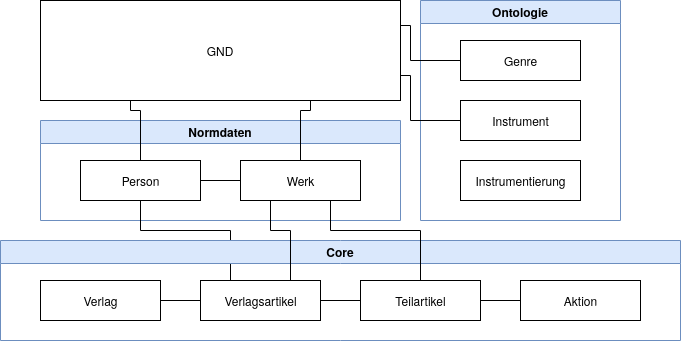
\includegraphics[scale=.45]{datenmodell}
}

\frame{\frametitle{Beispiel}
    \hspace{-2em}
    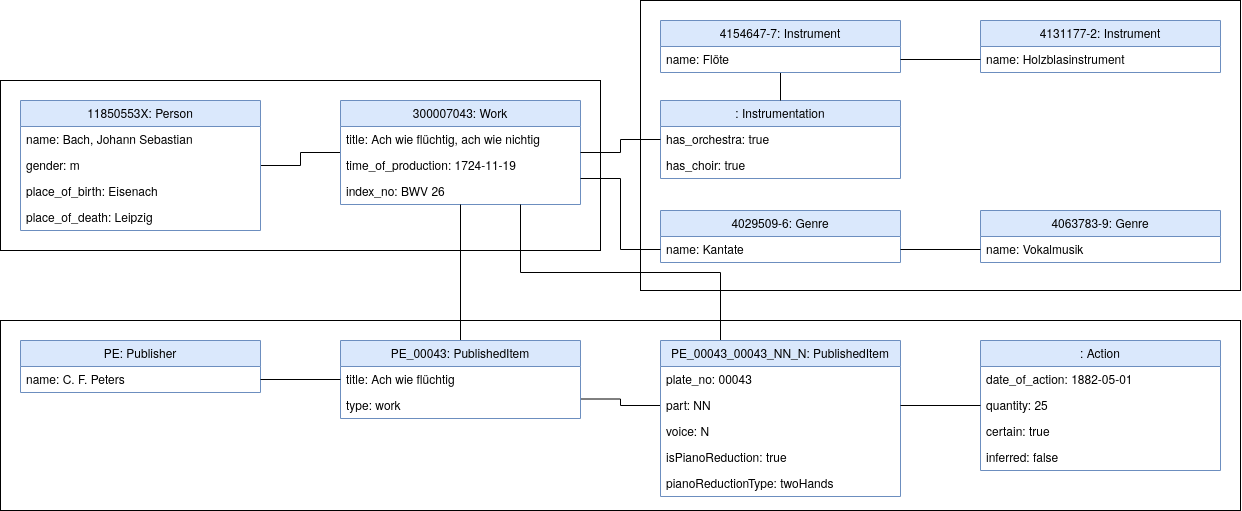
\includegraphics[scale=.26]{beispiel}
}

\frame{\frametitle{Architektur}
    \hspace{-2em}
    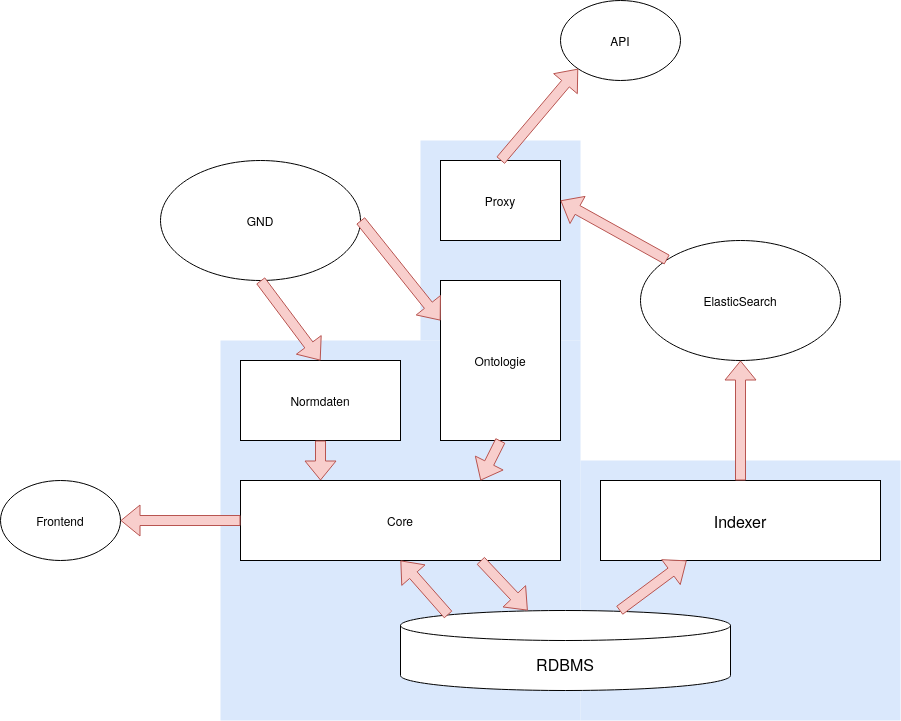
\includegraphics[scale=.3]{architektur}
}

\section{Einführung Statistik}

\frame{\frametitle{Skalen}
    \begin{itemize}
        \item Nominalskalen \\
            Verlagsartikeltyp
        \item Ordinalskalen \\
            Schulnoten
        \item Intervallskalen \\
            Datum
        \item Verhältnisskalen \\
            Auflagenhöhe
    \end{itemize}
}

\section{Visualisierungen}

\section{Inferentielle Statistik}

\end{document}
